%!TEX ROOT=../dissertation.tex
% UZAVŘENO! ÚPRAVY JEN ŽIVOTNĚ NUTNÉ NEBO VE ZBYLÉM ČASE

\chapter{Introduction}
\label{chap:intro}
\section{Motivation}
\label{sec:motivation}

\begin{figure}
\centering
 \fbox{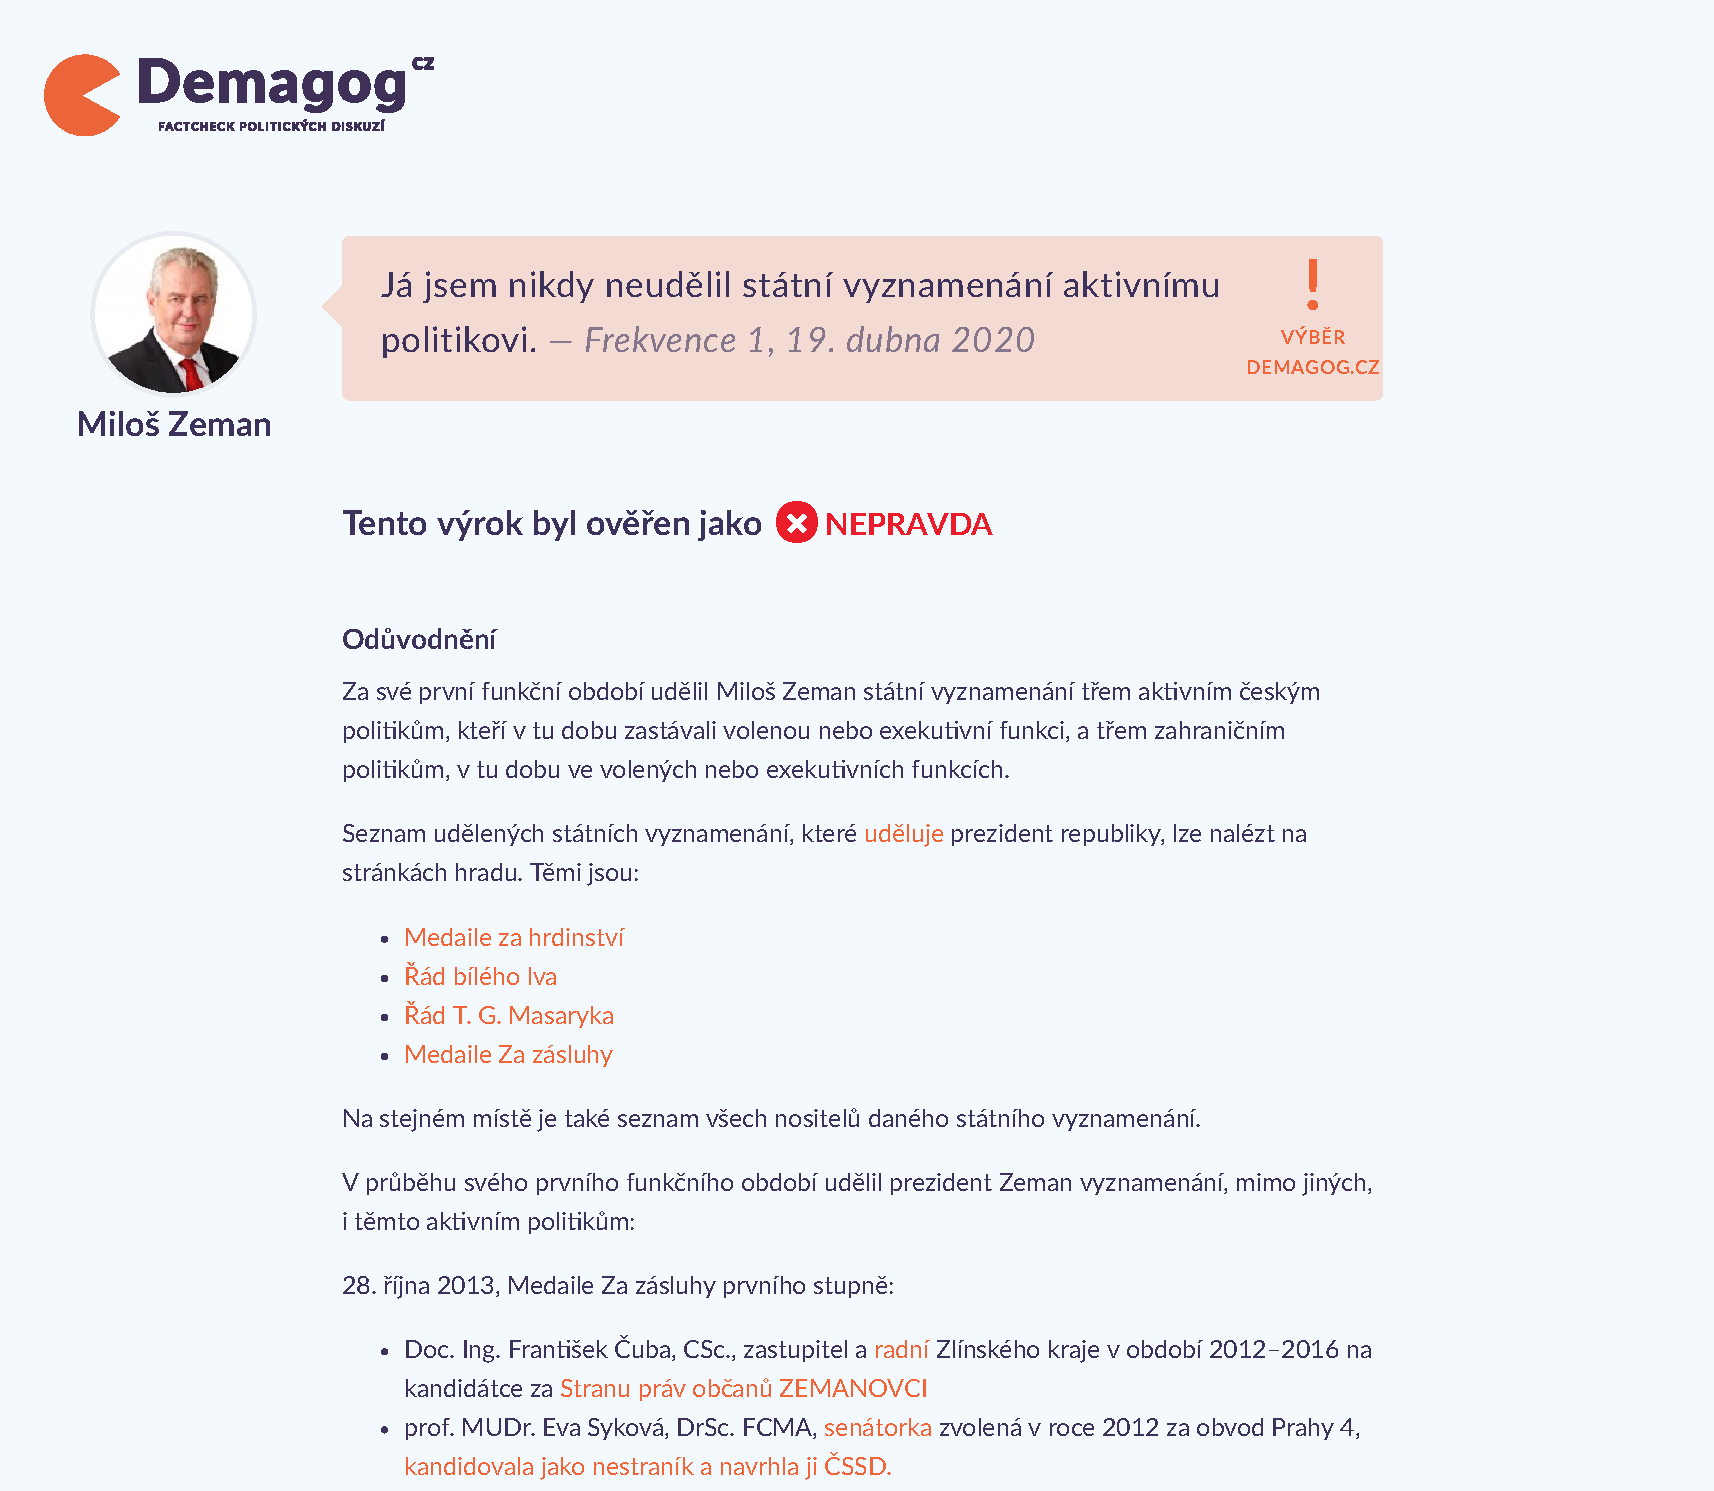
\includegraphics[width=\textwidth]{fig/demagog.pdf}}
\caption[Example fact verification from Czech portal Demagog.cz]{Example fact verification from Czech portal \textsf{Demagog.cz}.\\
Full annotation at \url{https://demagog.cz/vyrok/19225} -- translated in Appendix~\ref{trans:demagog}}
\label{fig:demagog}
\end{figure}
The spread of misinformation in the online space has a growing influence on the Czech public~\cite{stem}. It has been shown to influence people's behaviour on the social networks~\cite{Lazer1094} as well as their decisions in elections~\cite{10.1257/jep.31.2.211}, and real-world reasoning, which has shown increasingly harmful during the COVID-19 pandemic~\cite{BARUA2020100119}.

The recent advances in artificial intelligence and its related fields, in particular the recommendation algorithms, have contributed to the spread of misinformation on social media~\cite{doi:10.1177/2056305119888654}, as well as they hold a large potential for automation of the false content generation and extraction of sensational attention-drawing headlines -- the \"{clickbait} generation~\cite{shukai}.

Recent research has shown promising results~\cite{fever2} in false claim detection for data in English, using a trusted knowledge base of true claims (for research purposes typically fixed to the corpus of \textsf{Wikipedia} articles), mimicking the \textit{fact-checking} efforts in journalism.

Fact-checking is a rigorous process of matching every information within a \textit{factic claim} to its \textit{evidence} (or \textit{disproof}) in trusted data sources to infer the claim veracity and verifiability. In exchange, if the trusted \textit{knowledge base} contains a set of \"{ground truths} sufficient to fully infer the original claim or its negation, the claim is labelled as {\techbf{supported}} or {\techbf{refuted}}, respectively. If no such \textit{evidence set} can be found, the claim is marked as {\techbf{unverifiable}}\footnote{Hereinafter labelled as \texttt{NOT ENOUGH INFO}, in accordance to related research.}.


\section{Challenges}
Despite the existence of end-to-end fact-checking services, such as \url{politifact.org} or \url{demagog.cz}, the human-powered approach shows weaknesses in its scalability. By design, the process of finding an exhaustive set of evidence that decides the claim veracity is much slower than that of generating false or misguiding claims. Therefore, efforts have been made to move part of the load to a computer program that can run without supervision.

The common research goal is a fact verification tool that would, given a claim, semantically search provided knowledge base (stored for example as a \textit{corpus} of some natural language), propose a set of evidence (e. g. $k$ semantically nearest paragraphs of the corpus) and suggest the final verdict (Figure \ref{fig:pipeline}). This would reduce the fact-checker's workload to mere adjustments of the proposed result and correction of mistakes on the computer side. 

The goal of the ongoing efforts of {\textsf{FactCheck}} team at {\textsf{AIC CTU}}, as addressed in the works of~\cite{rypar,dedkova} and~\cite{gazo} is to explore the state-of-the-art methods used for fact verification in other languages, and propose a strong baseline system for such a task in Czech.

\subsection{Challenge subdivision}
\label{sec:subdivision}
In order to maximize our efficiency and the depth of our understanding of every relevant subproblem, we have divided the fact-checking task according to the Figure~\ref{fig:pipeline} among the members of our research group. 

The works of \cite{rypar} and~\cite{dedkova} focus on the Document Retrieval task and compare the performance of the numerical methods, s.a the \textit{tf--idf} search and the \textit{bag-of-words}, to the neural models, most notably the state-of-the-art \textit{Transformer networks}\cite{vaswani}. \cite{gazo} is proposing the methods of their scaling for long inputs, such as full news reports.

\subsection{Our contribution}
Our part is to provide the needed datasets for the fact verification tasks in the \textit{low-resource} Czech language. We examine both major ways of doing so -- localizing the large-scale datasets available in the high-resource languages, typically in English, and collecting a novel dataset through human annotation experiments.

Our second task is to establish a baseline for the final task of the fact-checking pipeline: the \textit{Natural Language Inference}, which is a decisioning problem of assigning a veracity verdict to a claim, given a restricted \textit{set of evidence} in the Czech natural language.

In continuation with research funded by \textsf{TAČR}, experiments are to be made using the archive of the \textsf{Czech News Agency} (hereinafter referred to as \textsf{ČTK}\footnote{Which stands for \"{\textsf{Česká Tisková Agentura}}, the original name of \textsf{Czech News Agency}}) for a knowledge base, exploring whether a corpus written using journalistic style can be used for such a challenge.



\section{A word on the Transformers}
\label{sec:transformers}
For the past four years, the state-of-the-art solution for nearly every Natural Language Processing task is based on the concept of \textit{transformer networks} or, simply, \textit{Transformers}. This has been a major breakthrough in the field by~\cite{vaswani}, giving birth to the famous models such as \textsf{Google}'s \textsf{BERT}~\cite{devlin2019bert} and its descendants, or the \textsf{OpenAI}'s \textsf{GPT-3}~\cite{gpt3}.

In our proposed methods, we use Transformers in every step of the fact verification pipeline. Therefore, we would like to introduce this concept to our reader to begin with. 

Transformer is a neural model for \textit{sequence-to-sequence} tasks, which, similarly e.g. to the \textit{LSTM-Networks}~\cite{lstm}, uses the Encoder--Decoder architecture. Its main point is that of using solely the \textit{self-attention} mechanism to represent its input and output, instead of any sequence-aligned recurrence~\cite{vaswani}.

In essence, the \textit{self-attention} (also known as the \textit{intra-attention}) transforms every input vector to a weighted sum of the vectors in its neighbourhood, weighted by their \textit{relatedness} to the input. One could illustrate this on the \textit{euphony} in music, where every tone of a song relates to all of the precedent ones, to some more than to the others.

The full Transformer architecture is depicted in Figure~\ref{fig:transformer}.
%--- FIG: UTF forms
\begin{figure}
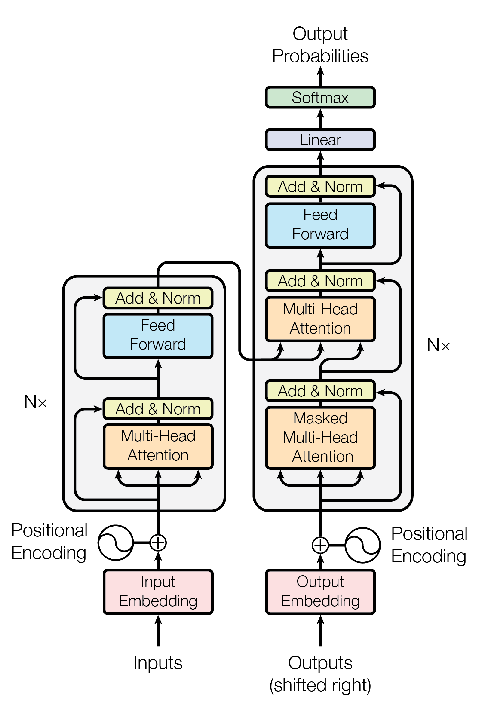
\includegraphics[width=9cm]{fig/transformer.pdf}
\caption{Transformer model architecture, reprinted from~\cite{vaswani}}
\label{fig:transformer}
\end{figure}
%--- /FIG



\section{Thesis outline}
Due to the bipartite nature of our thesis assignment, we have divided the chapters to follow into two parts. The {\techbf{Part~\ref{parti}}} presents our Czech datasets and the methods of their collection, and the {\techbf{Part~\ref{partii}}} makes the initial experiments for the NLI task.
\begin{itemize}
\item {\techbf{Chapter~\ref{chap:intro}}} introduces the problem, motivates the research on the topic and sets up the challenges of this thesis 

\item {\techbf{Chapter~\ref{chap:collection}}} examines the most relevant research in the field, with an emphasis on the methods of dataset collection, it introduces the two subsequent chapters on the topic

\item {\techbf{Chapter~\ref{chap:fever_cs}}} lists and justifies our methods of generating the \textit{localized dataset}, i. e. the methods of transferring the learning examples from a high-resource Natural Language to Czech

\item {\techbf{Chapter~\ref{chap:ctk}}} describes our methods of collecting a novel fact-checking dataset using the non-encyclop\ae dically structured knowledge base of \textsf{ČTK} news reports

\item {\techbf{Chapter~\ref{chap:dataset}}} introduces the resulting dataset, as collected during three waves of annotation with Václav Moravec and students of the \textsf{Faculty of Social Sciences}
% Experiments
\item  {\techbf{Chapter~\ref{chap:pipeline}}} briefly introduces the full fact-checking pipeline we have established with the \textsf{FactCheck} team at \textsf{AIC} using the collected data and a couple of real-world applications stemming from it
\item {\techbf{Chapter~\ref{chap:nli}}} explores the state-of-the-art methods of Natural Language Inference and their potential for our system, and it proceeds to make preliminary experiments on our dataset using these methods
\item Finally, {\techbf{Chapter~\ref{chap:conclusion}}} concludes the thesis, summarises the results we have achieved and proposes directions for future research

\end{itemize}

